\chapter{Rings}\label{chap:rings}
\section{Introduction to Rings}
\subsection{Definitions and Examples}
\begin{definition}[Ring]
A \vocab{ring}\index{ring} $(R,+,\times,0,1)$ consists of a set $R$, $0,1\in R$, together with two binary operations addition and multiplication, denoted $+$ and $\times$, satisfying the following axioms:
\begin{enumerate}[label=(\roman*)]
\item $(R,+)$ is an abelian group with additive identity $0$.
\item $\times$ is associative with multiplicative identity $1$.
\item $\times$ distributes over $+$: for all $a,b,c\in R$,
\begin{align*}
a\times(b+c)&=(a\times b)+(a\times c),\\
(a+b)\times c&=(a\times c)+(b\times c).
\end{align*}
\end{enumerate}
\end{definition}

\begin{notation}
We simply write $ab$ rather than $a\times b$ for $a,b\in R$.
\end{notation}

A ring is said to be a \vocab{commutative ring} if $\times$ is commutative.

\begin{remark}
It is also worth noting that some texts require an additional axiom asserting that $1\neq0$. In fact it is easy to see from the other axioms that if 1 = 0 then the ring has only one element. We will refer to this ring as the ``zero ring''. While it is a somewhat degenerate object, it seems unnecessary to me to exclude it.
\end{remark}

\begin{definition}
A ring $R$ with identity $1$, where $1\neq0$, is called a \vocab{division ring}\index{ring!division ring} if every $a\in R$, $a\neq0$ has a multiplicative inverse, i.e. there exists $b\in R$ such that $ab=ba=1$.

A commutative division ring is called a \vocab{field}\index{ring!field}.
\end{definition}

\begin{figure}[H]
\centering
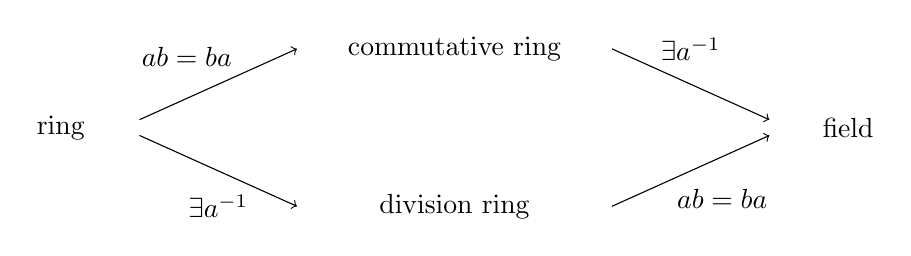
\begin{tikzpicture}
\node at (-0.5,0) {ring};
\draw[->] (0.5,0.1) -- (2.5,1);
\node at (1.1,0.9) {$ab=ba$};
\node at (4.5,1) {commutative ring};
\draw[->] (0.5,-0.1) -- (2.5,-1);
\node at (1.5,-1) {$\exists a^{-1}$};
\node at (4.5,-1) {division ring};
\draw[->] (6.5,1) -- (8.5,0.1);
\node at (7.5,1) {$\exists a^{-1}$};
\draw[->] (6.5,-1) -- (8.5,-0.1);
\node at (7.9,-0.9) {$ab=ba$};
\node at (9.5,0) {field};
\end{tikzpicture}
\end{figure}

\begin{example}
$\ZZ$ under usual addition and multiplication is a commutative ring with identity $1$.

$\QQ$, $\RR$, $\CC$ are field.

$\ZZ/n\ZZ$ is a commutative ring with identity $\bar{1}$ under addition and multiplication of residue classes.
\end{example}

\begin{proposition}
Let $R$ be a ring. Then
\begin{enumerate}[label=(\roman*)]
\item $0a=a0=0$ for all $a\in R$.
\item $(-a)b=a(-b)=-(ab)$ for all $a,b\in R$.
\item $(-a)(-b)=ab$ for all $a,b\in R$.
\item if $R$ has identity $1$, then the identity is unique and $-a=(-1)a$.
\end{enumerate}
\end{proposition}

\begin{proof}
These all follow from the distributive laws and cancellation in the additive group $(R,+)$.
\begin{enumerate}[label=(\roman*)]
\item $0a=(0+0)a=0a+0a$ then add the additive identity of $0a$ to both sides to get $0a=0$. Similarly, $a0=a(0+0)=a0+a0$ then add the additive identity of $a0$ to both sides to get $a0=0$.
\item 
\item 
\item 
\end{enumerate}
\end{proof}

\begin{definition}[Subring]
$S\subset R$ is a \vocab{subring}\index{ring!subring} of ring $R$ if $S$ is a subgroup of $R$ that is closed under multiplication.
\end{definition}

\begin{lemma}[Subring criterion]
Let $R$ be a ring, $S\subset R$. Then $S$ is a subring of $R$ if and only if
\begin{enumerate}[label=(\roman*)]
\item $1\in S$;
\item $s_1s_2\in S$ and $s_1-s2\in S$ for all $s_1,s_2\in S$.
\end{enumerate}
\end{lemma}

\begin{proof} \

\fbox{$\implies$}

\fbox{$\impliedby$} The condition that $s_1-s_2\in S$ for all $s_1,s_2\in S$ implies that $S$ is an additive subgroup by the subgroup test (note that as $1\in S$ we know that $S$ is nonempty). The other conditions for a subring hold directly.
\end{proof}

When studying any kind of algebraic object, it is natural to consider maps between those kind of objects which respect their structure. For example, for vector spaces the natural class of maps are linear maps, and for groups the natural class are the group homomorphisms. The natural class of maps to consider for rings are defined similarly:

\begin{definition}
Let $R$ and $S$ be rings. $\phi:R\to S$ is a \vocab{homomorphism}\index{homomorphism} if it satisfies
\begin{enumerate}[label=(\roman*)]
\item $\phi(1_R)=1_S$;
\item $\phi(r_1+r_2)=\phi(r_1)+\phi(r_2)$ for all $r_1,r_2\in R$;
\item $\phi(r_1r_2)=\phi(r_1)\phi(r_2)$ for all $r_1,r_2\in R$.
\end{enumerate}
A bijective ring homomorphism is called an \vocab{isomorphism}\index{isomorphism}, denoted by $R\cong S$.
\end{definition}

Recall that in a ring we do not require that nonzero elements have a multiplicative inverse. Nevertheless, because the multiplication operation is associative and there is a multiplicative identity, the elements which happen to have multiplicative inverses form a group:

\begin{definition}[Unit]
Let $R$ be a ring. $a\in R$ is called a \vocab{unit} in $R$ if there exists $b\in R$ such that $ab=ba=1$.
\end{definition}

\begin{proposition}
The units in a ring $R$ form a group under multiplication.
\end{proposition}

\begin{definition}[Group of units]
Let $R$ be a ring. The subset
\[R^\times = \{r\in R\mid \exists s\in R, rs=1\}\]
is called the \vocab{group of units} in $R$; it is a group under multiplication $\times$ with identity element $1$.
\end{definition}

\subsection{Polynomial Rings}

\section{Basic Properties}
\subsection{Integral Domains}
\begin{definition}
Let $R$ be a ring. $a\in R\setminus\{0\}$ is called a \vocab{zero divisor}\index{zero divisor} if there exists $b\in R\setminus\{0\}$ such that $ab=0$.

A ring which is not the zero ring and has no zero divisors is called an \vocab{integral domain}\index{integral domain}. Thus if a ring is an integral domain and a.b = 0 then one of a or b is equal to zero.
\end{definition}

The absence of zero divisors in integral domains give these rings a cancellation property:

\begin{proposition}
Let $R$ be a ring. $a,b,c\in R$, $a$ is not a zero divisor. If $ab=ac$, then either $a=0$ or $b=c$. In particular, for any $a,b,c$ in an integral domain and $ab=ac$, then either $a=0$ or $b=c$.
\end{proposition}

\begin{corollary}
Any finite integral domain is a field.
\end{corollary}

\subsection{The Field of Fractions}

\section{Ideals and Quotients}
From now on we will assume all our rings are commutative. In this section we study the basic properties of ring homomorphisms, and establish an analogue of the ``first isomorphism theorem'' which you have seen already for groups. Just as for homomorphisms of groups, homomorphisms of rings have kernels and images.

\begin{definition}
Let $\phi:R\to S$ be a ring homomorphism. The \vocab{kernel} of $\phi$ is
\[\ker\phi\coloneqq\{r\in R\mid\phi(r)=0\},\]
and the \vocab{image} of $\phi$ is
\[\im\phi\coloneqq\{s\in S\mid \exists r\in R, \phi(r)=s\}.\]
If $\im\phi=S$, we say that $\phi$ is surjective.
\end{definition}

\begin{definition}
Let $R$ be a ring. A subset $I\subset R$ is called an \vocab{ideal} in $R$, denoted by $I\triangleleft R$, if
\begin{enumerate}[label=(\roman*)]
\item $I$ is a subgroup of $(R,+)$;
\item $ar\in I$ for all $a\in I$, $r\in R$.
\end{enumerate}
\end{definition}

\begin{lemma}
If $\phi:R\to S$ is a ring homomorphism, then $\ker\phi$ is an ideal. Moreover $I\subset R$ is an ideal if and only if it is nonempty, closed under addition, and closed under multiplication by arbitrary elements of $R$.
\end{lemma}

\begin{proof}
This is immediate from the definitions. For the moreover part, we just need to check that $I$ is closed under taking additive inverses. But this follows from the fact that it is closed under multiplication by any element of $R$ since $-x=(-1)x$ for any $x\in R$.
\end{proof}

Note that if $I$ is an ideal of $R$ which contains $1$, then $I=R$. We will shortly see that in fact any ideal is the kernel of a homomorphism. First let us note a few basic properties of ideals:


\section{Domains}
\subsection{Euclidean Domains}
\subsection{Principal Ideal Domains}
\subsection{Unique Factorisation Domains}

\section{Polynomial Rings}


%Ideals, quotient rings, isomorphism theorems. Prime and maximal ideals. Field of fractions of an integral domain. Factorization in rings; units, primes and irreducibles. Unique factorization in principal ideal domains, and in polynomial rings. Gauss’ Lemma and Eisenstein’s irreducibility criterion. Rings $\ZZ[\alpha]$ of algebraic integers as subsets of $\CC$ and quotients of $\ZZ[x]$. Examples of Euclidean domains and uniqueness and non-uniqueness of factorization. Factorization in the ring of Gaussian integers; representation of integers as sums of two squares. Ideals in polynomial rings. Hilbert basis theorem